\label{sec:mountain_car}
In the mountain car problem we start at the bottom of a valley the goal is to reach the top of the mountain on the right (see \autoref{fig:mcar}). On the left side is a wall that simply blocks the agent. For each time step an agent can choose to give the car some impulse to the left, to the right or do nothing. This task seems trivial however the car is under powered, simply going right all the time will not bring you to the top. As a human you would quickly figure out that you need to swing between the walls higher and higher to build up momentum just as if you where on a swing in a children's playground. However the agent will get far less information. 

\begin{marginfigure}
    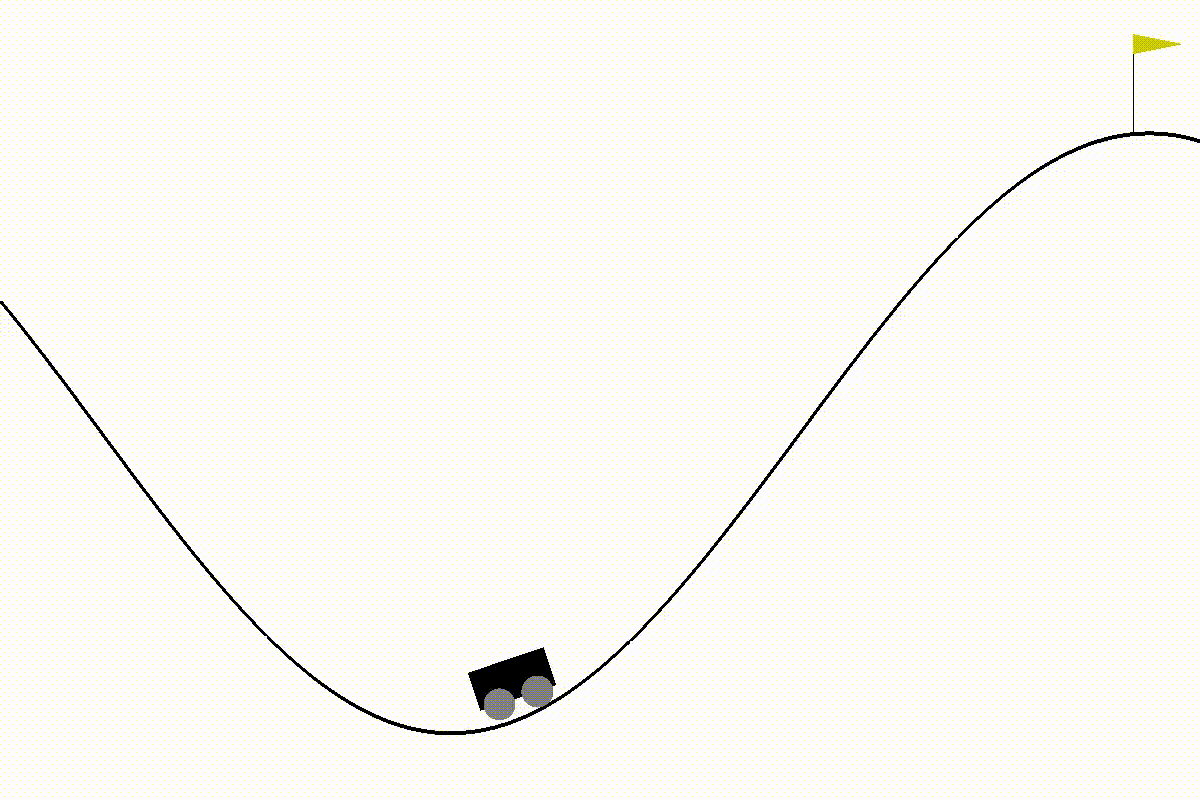
\includegraphics{mcar}
    \caption{The mountain car problem after the agent has taken an action to the right}
    \label{fig:mcar}
\end{marginfigure}

The agent gets a reward \textit{only} when the task has been completed. It gets punished for every time step the task is not completed. The only thing it gets next to this feedback is the current state of the car, its location and its velocity. Here I use DQN to get the car to perform the task. In the beginning it will perform random actions learning features of the environment, once it succeeds it will try to replicate that behavior eventually learning how to optimally reach the goal.

\subsection{Implementation}
\label{sec:mcar_impl}
This implementation of DQN implements both the essential replay buffer and infrequent weight updates for the neural network. The agent gets 1000 attempts to perform the task, we shut an attempt down after 200 time steps. Each session starts by requesting an action from the network or taking a random step, this is governed by the rate of random actions $\epsilon$ which we decrease during training. The action is then performed on the environment, we use the implementation of mountain car provided by the \textit{openAI gym} project, specifically we use \texttt{MountainCar-v0}. The environment returns the state after the action has been performed, the reward and weather the task is done. We add the before and after state together with the reward and weather the task is done to memory. Then if the memory has enough experience (400 samples) we train the network before starting over for the next step. This continues until the task is completed or the maximum number of steps is reached. After each training step we copy the weights from the training network to the predicting network as motivated in \autoref{sec:infrequent_weight_updates}. 

The memory, network and random step rate epsilon are implemented as python classes: \texttt{Memory}, \texttt{Predictor} and \texttt{Epsilon}. 

The \texttt{Memory} class uses a deque to store events that consist of the \textit{before} and \textit{after} state together with the \textit{score} and if the \textit{game is over}. It has a member function to add such an event, a sample method to return a random sample of events and a length member which is used to determine weather the memory has enough experience to start training the network. The memory forgets old events keeping track of only the last $20 000$ events.

The \texttt{Predictor} wraps around a simple three layer neural network implemented using Keras\cite{keras}, it provides a subset of the Keras api: \texttt{predict()}, \texttt{fit()} as well as methods for infrequent weight updates: \texttt{copy\_weights\_from(self, other)} and \texttt{clone(self)}. The first two functions help reshape the data using numpy\cite{numpy}. The network consists of two hidden layers, an input of size 2 encoding the position and velocity as floats, and an output layer of size 3 that encodes the Q-score for each action, of which there are 3 (left, right or nothing).
The first hidden layer has 24 fully connected nodes and the second 48. Both hidden layers use the \textit{rectified linear unit} as activation function however the output layer uses a linear activation function. The network uses the \textit{mean square error} as loss and optimizes using the \textit{Adam} optimizer as it is suitable for noisy and sparse gradients.

The \texttt{Epsilon} class provides a decaying random action ratio. It starts with value $1$ which translates as only take random actions. Every time the \texttt{decay} method is called the epsilon value is decreased slightly (by $5^{-5}$) until a minimal value of $0.01$ is reached which means the agent takes a random action for only 1\% of steps. As we call \texttt{decay} every time we take an action $\epsilon$ linearly decays from $1$ to $0.01$.

The network trains using experience replay by taking $32$ samples from the replay buffer and training on them. For each sample the input for the neural network is the state before an action was applied, the \textit{before state}. The labels are however not the Q-values. The learning rate from the classic Q-formula (\autoref{eq:Q} in \autoref{sec:theory}) is applied by the learning of the network. The old Q-value is encoded in the existing network and incorporated in that way. The labels are then the part of the Q-formula not already implemented in the training: the reward $r_t$ plus the discount factor $\gamma$ and the estimate of the future Q value ${max}_a Q(s_{t+1},a)$. Gamma is $0.95$ for this implementation. The estimate is given by the output of the network for the after state and the reward is the score. When the game has ended it does no longer make sense to incorporate future results in the Q-value, in that case we let the label be the current score and do not add $\gamma$ times the Q-value for the \textit{after} state. As the output of the network is the Q-value of all possible actions and we only know how to update the Q-value for the action that was taken we use the current predicted Q-values for the other actions. 

To speed up the learning of the network I minimized the calls to \textit{keras} functions by doing the predictions and learning for the entire batch. We first calculate the Q-values for all the \textit{before states} and the \textit{after states} in the sample. Then looping over the samples we use the just calculated Q-values to find the labels as described above. Finally we do the training of the network for the entire batch again.